\documentclass[tikz,border=0mm]{standalone}
\usepackage[T1]{fontenc}
\usepackage[swedish,english]{babel}
\usepackage{amsmath}
\usepackage{tikz}
\usepackage{amssymb}
\usetikzlibrary{shadows}
\usetikzlibrary{arrows,positioning}
\usepackage{pgfplots}
\usepgfplotslibrary{colormaps}%
\usetikzlibrary{backgrounds}
%\newcommand\HUGE{\@setfontsize\Huge{48}{57}} 
\makeatletter
\newcommand\HUGE{\@setfontsize\Huge{90}{100}}
\makeatother   
\makeatletter
\newcommand\hugest{\@setfontsize\Huge{110}{120}}
\makeatother   
%\pgfplotsset{%
%    colormap={paraviewMap}{rgb255=(0.231371,0.298039,0.752941) rgb255=(0.865003,0.865003,0.865003) rgb255=(0.705882,0.0156863,0.14902)}%
%}%   
\pgfplotsset{
  every axis/.style = {
    colormap name = viridis,
    opacity = 0.3,
  },
}
\definecolor{mycolor}{RGB}{255,51,76}

% THE PICTURE BEGINS
\begin{document}
\begin{tikzpicture}[show background rectangle,background rectangle/.style={fill=white}]

%====================================================================
% Classic
\node[inner sep=0pt] at (-9,0)
    {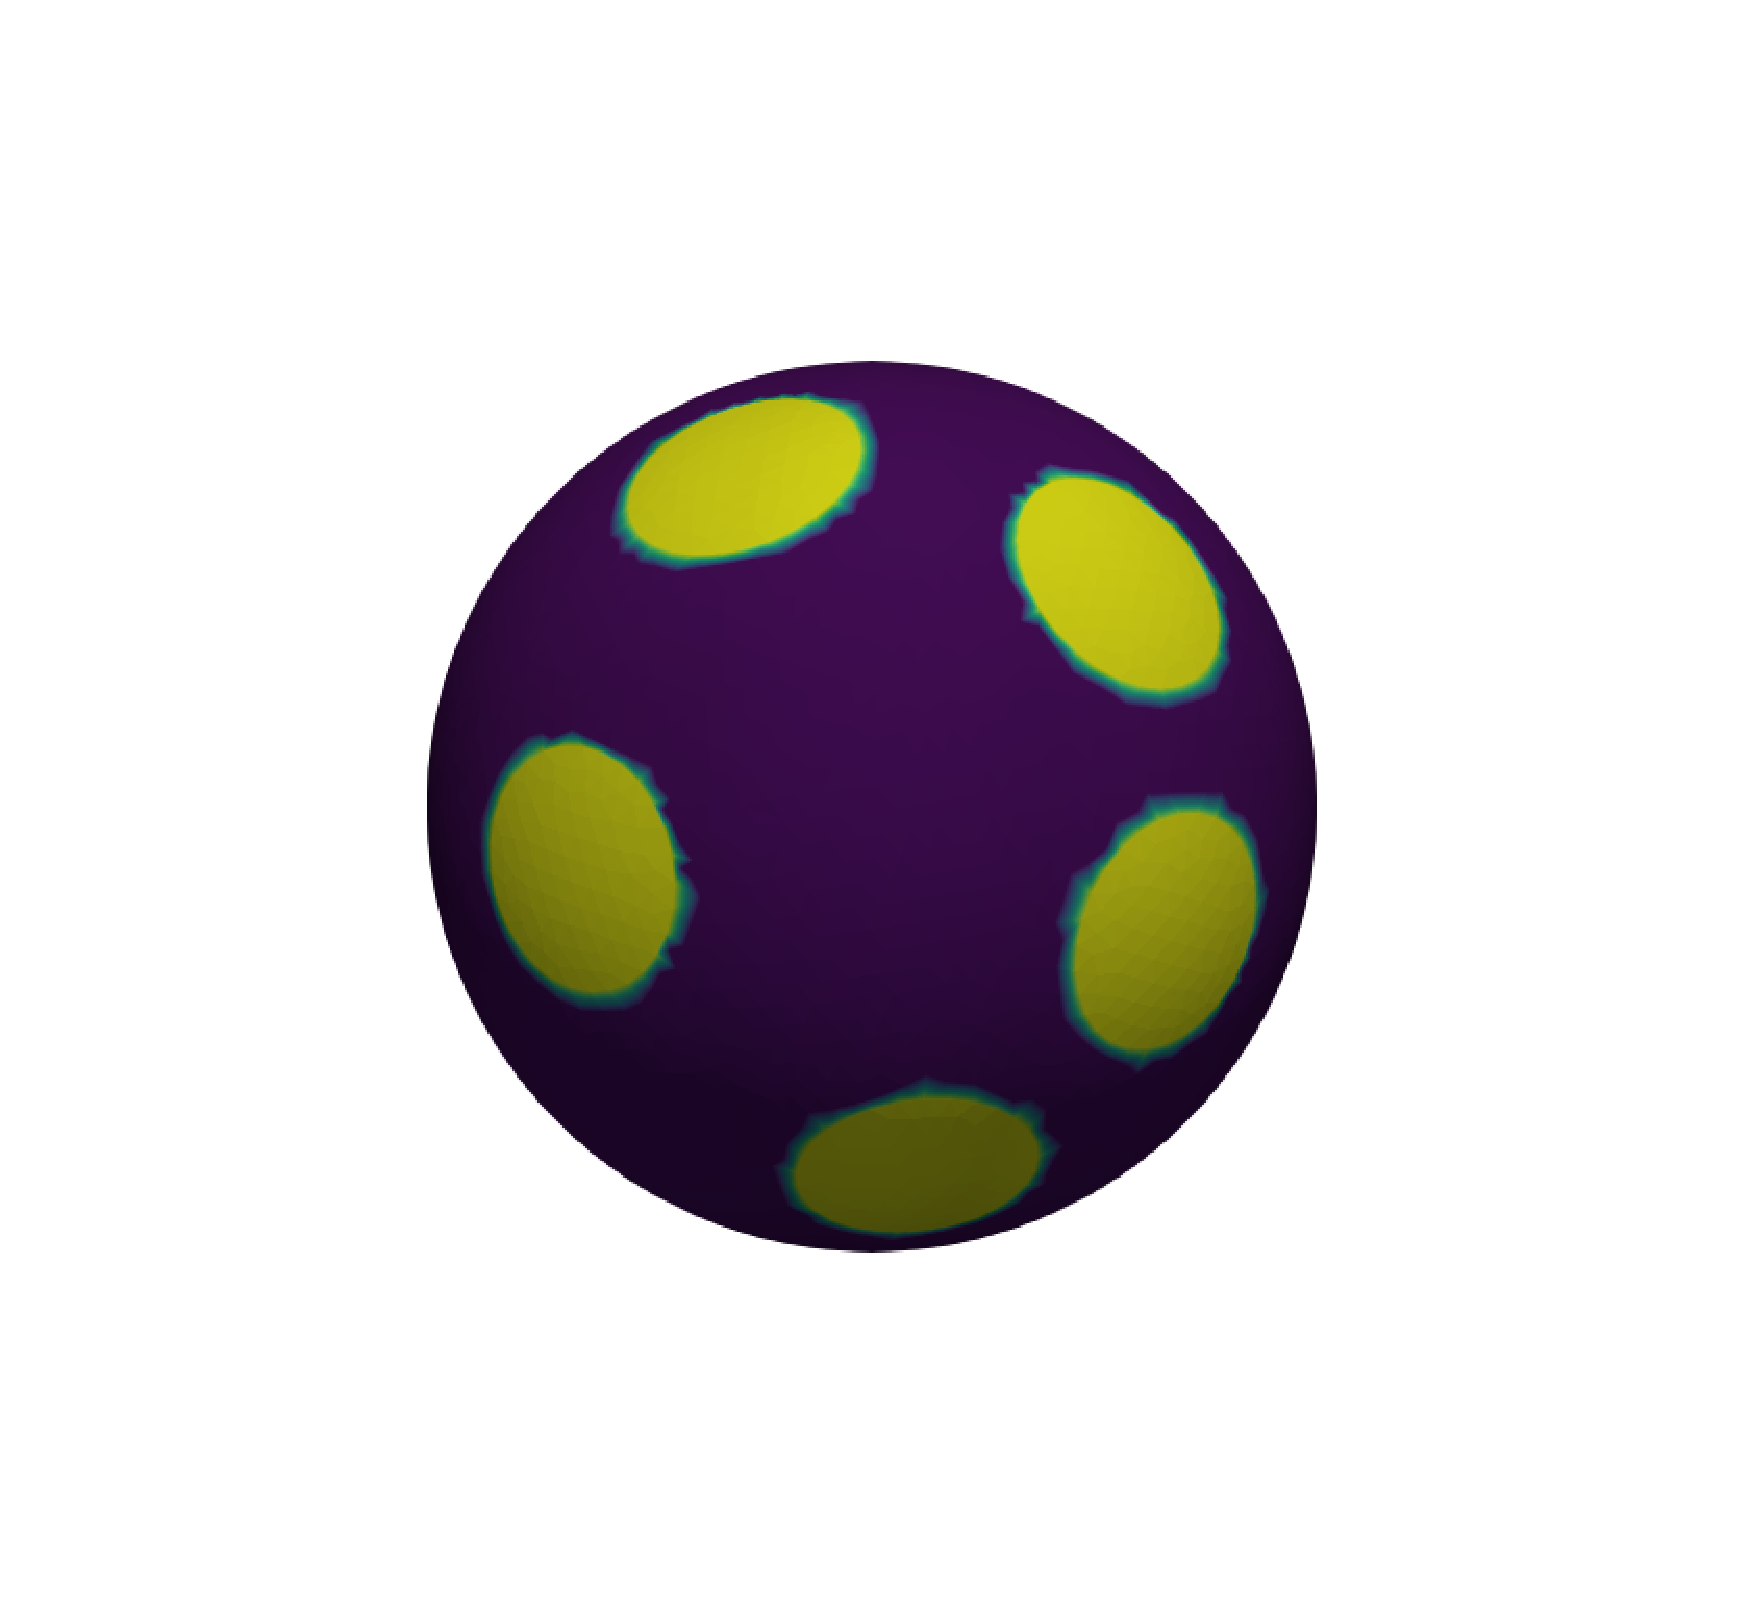
\includegraphics[scale=0.178]{./Pictures/v0.eps}};
% Non-classic
\node[inner sep=0pt] at (-9,-6)
    {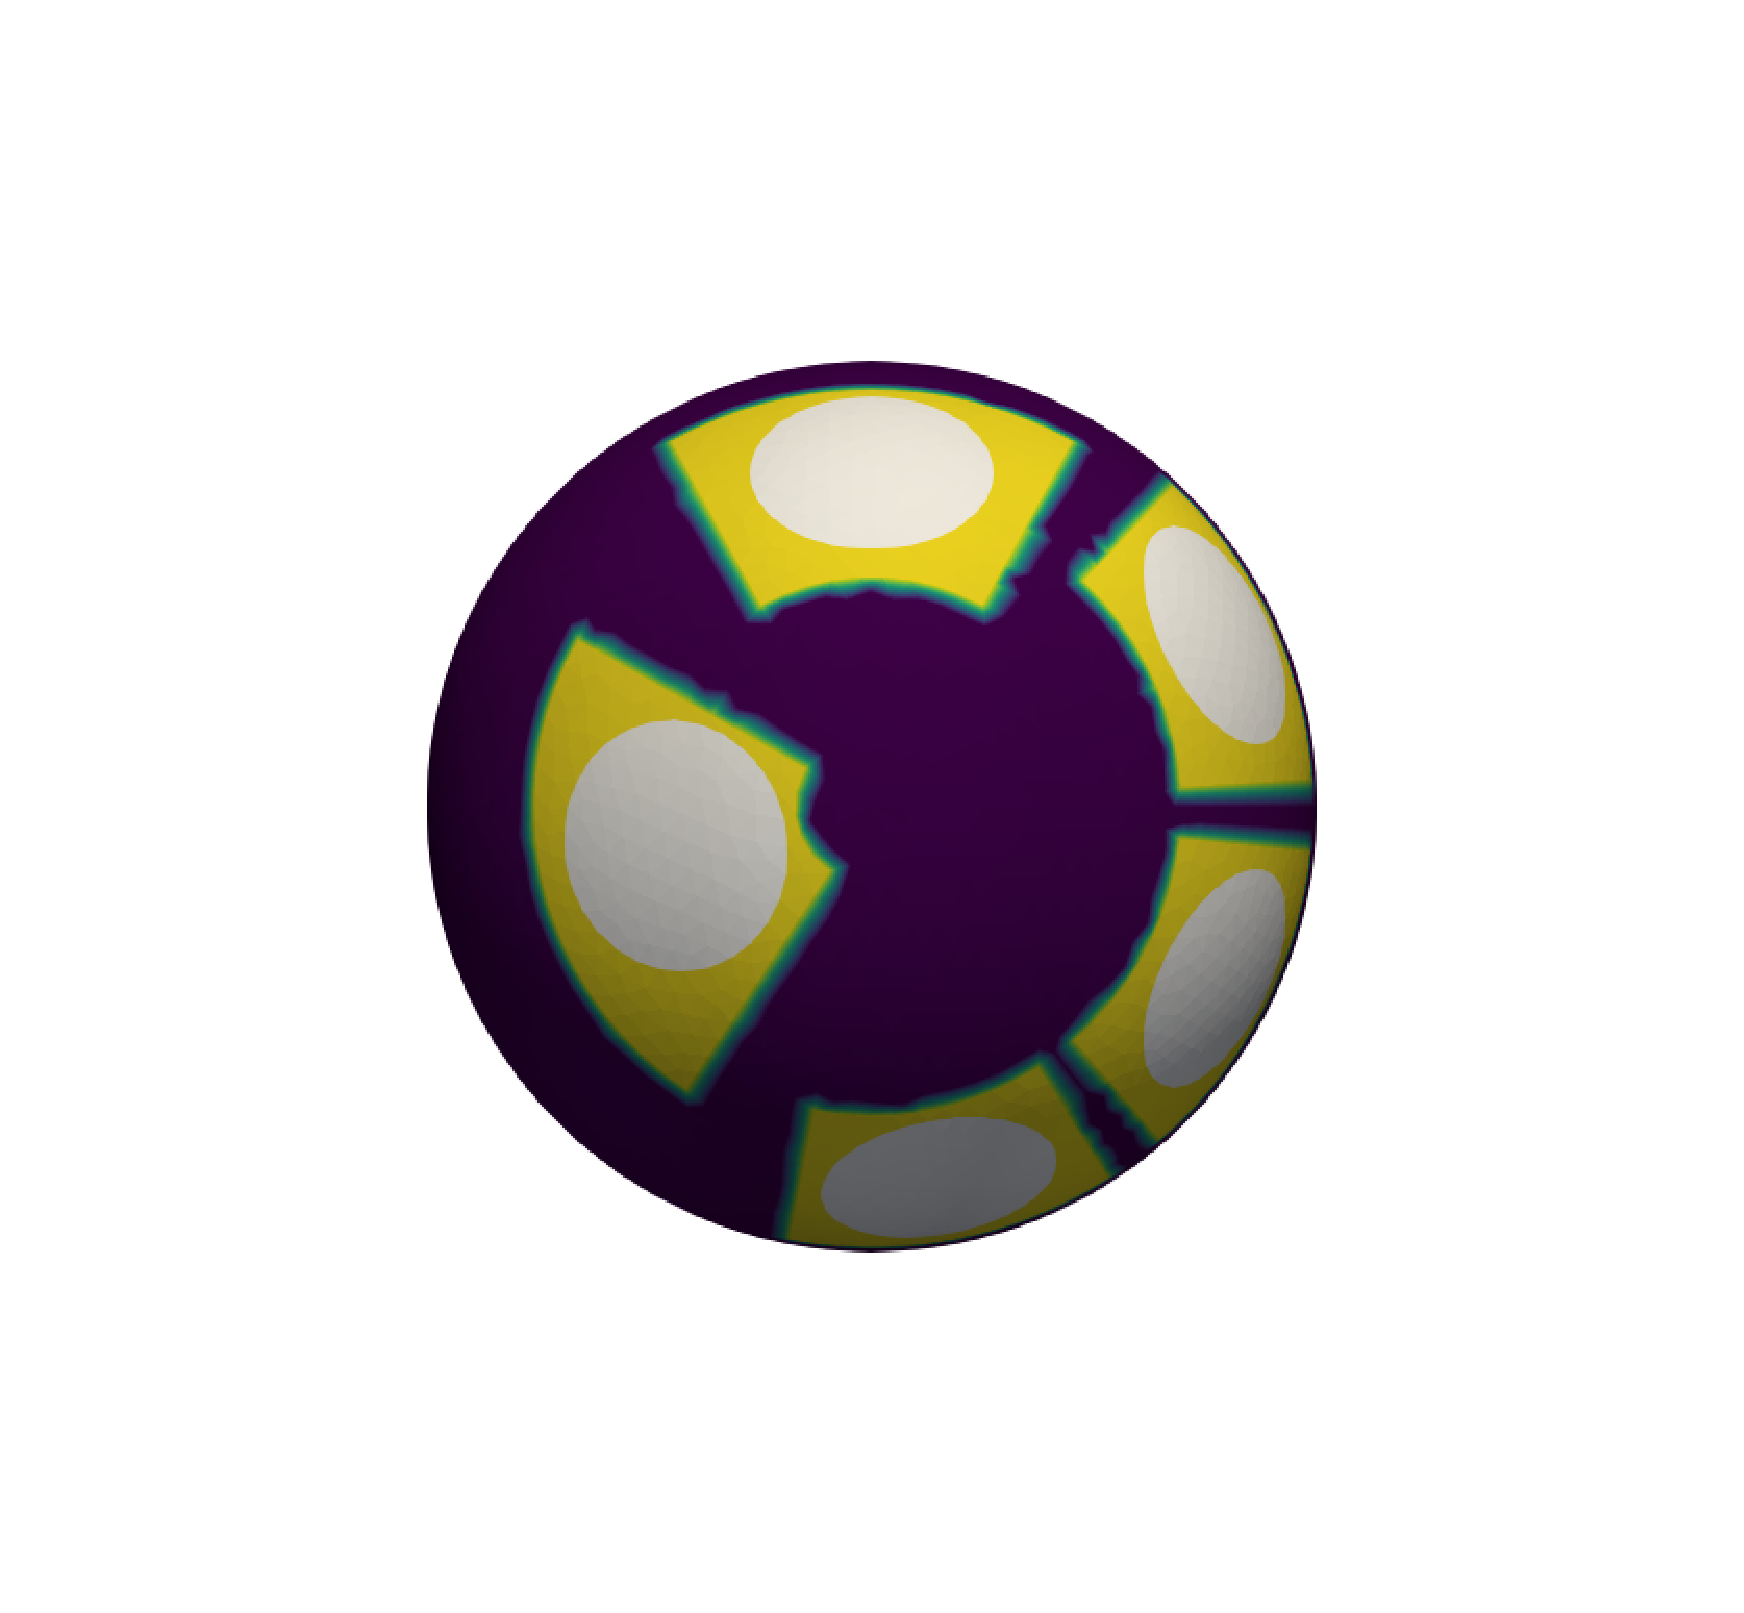
\includegraphics[scale=0.178]{./Pictures/p0.eps}};
%====================================================================
% Classic
\node[inner sep=0pt] at (-3,0)
    {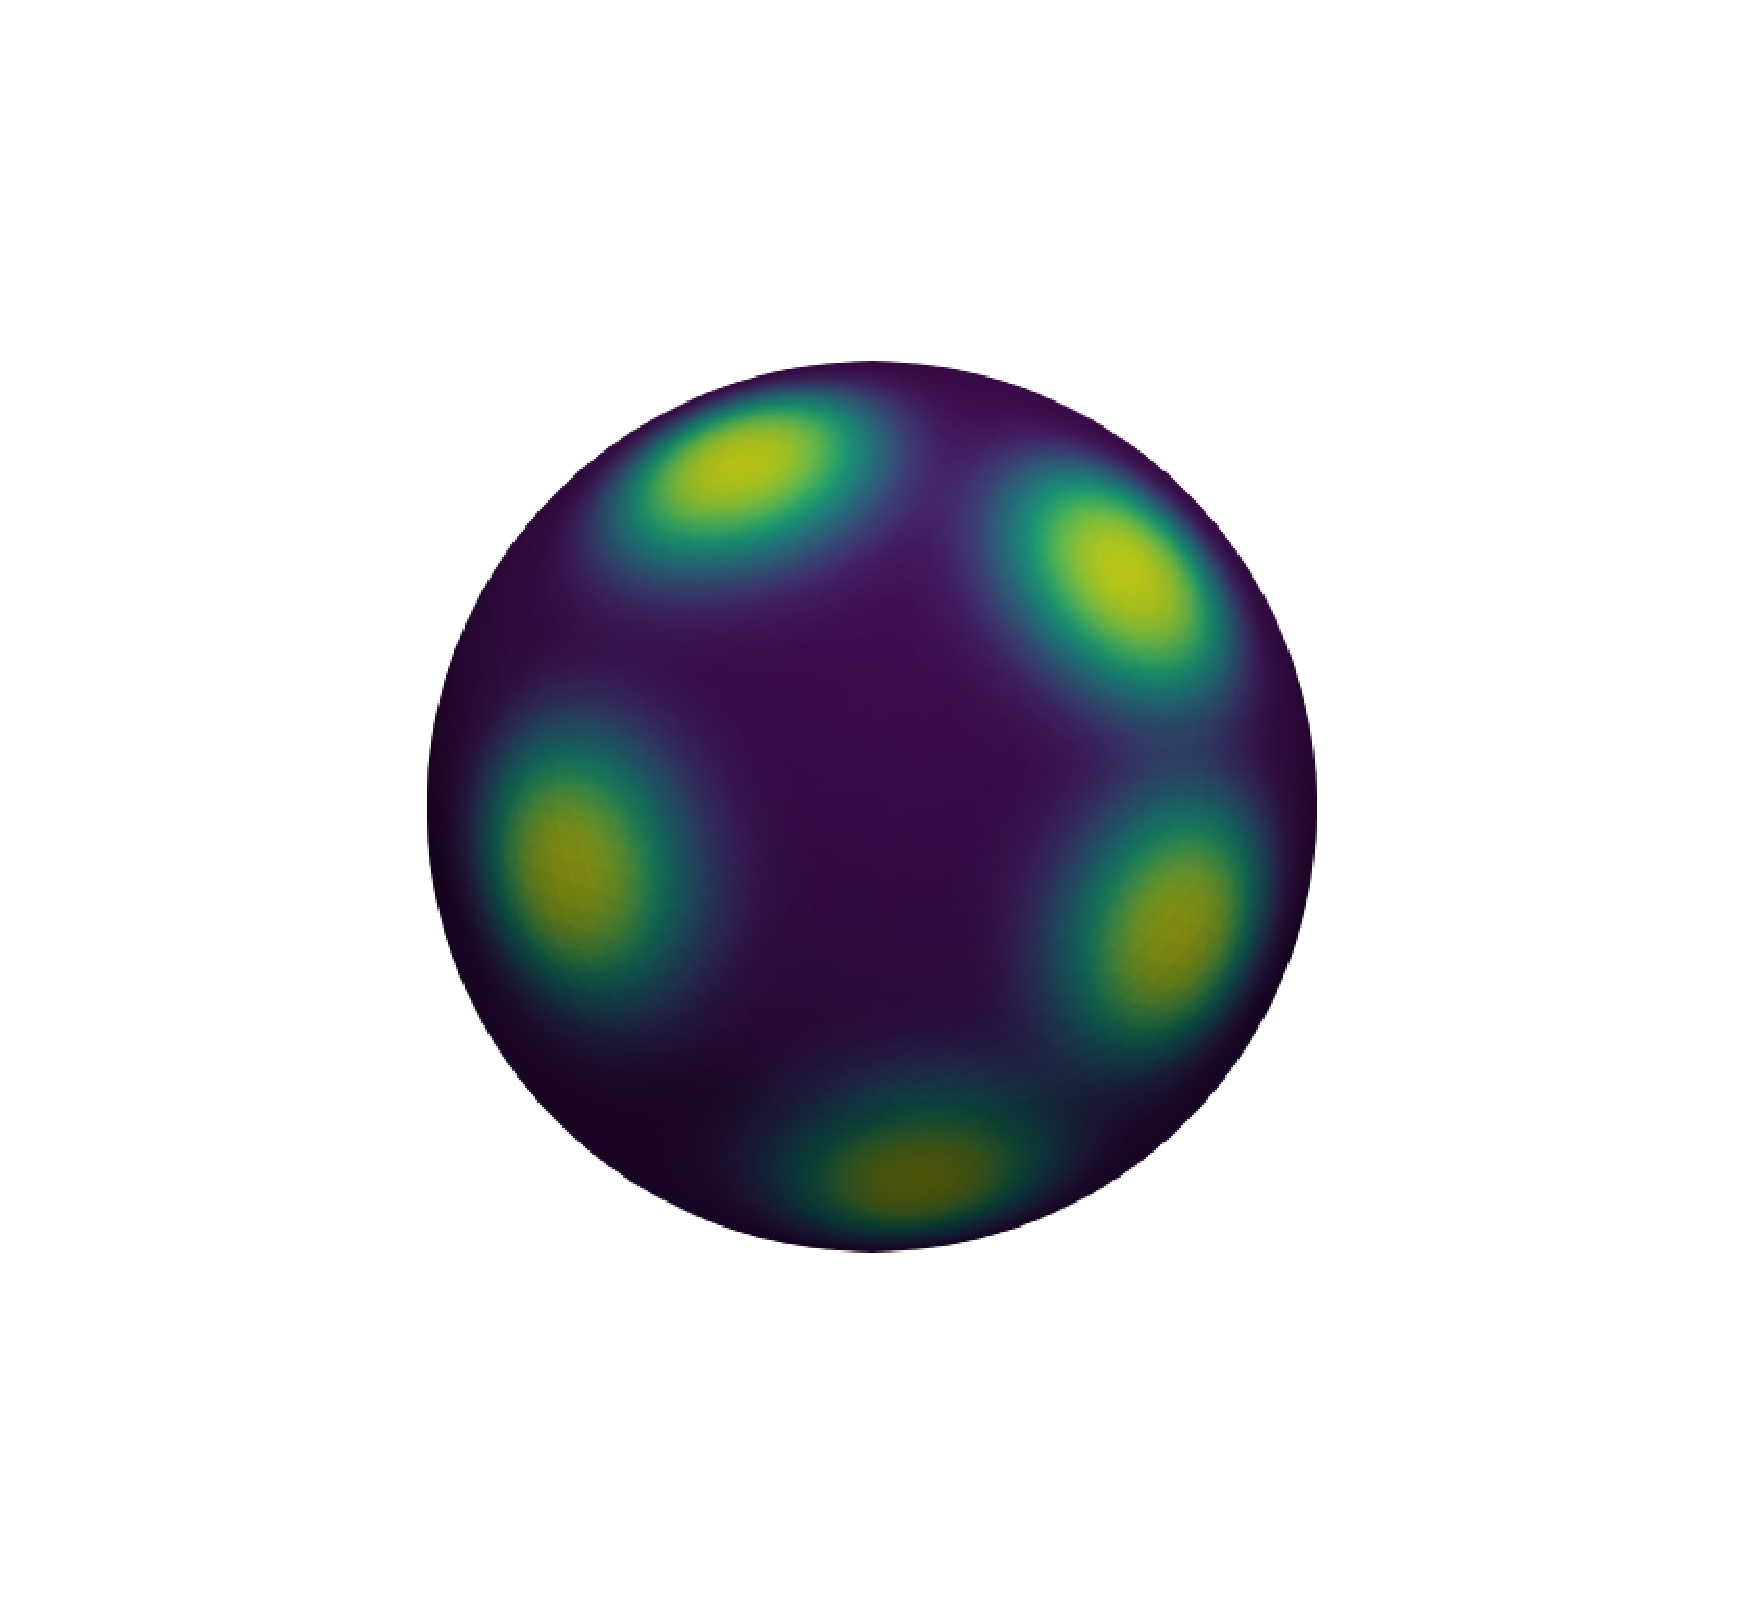
\includegraphics[scale=0.178]{./Pictures/v1.eps}};
% Non-classic
\node[inner sep=0pt] at (-3,-6)
    {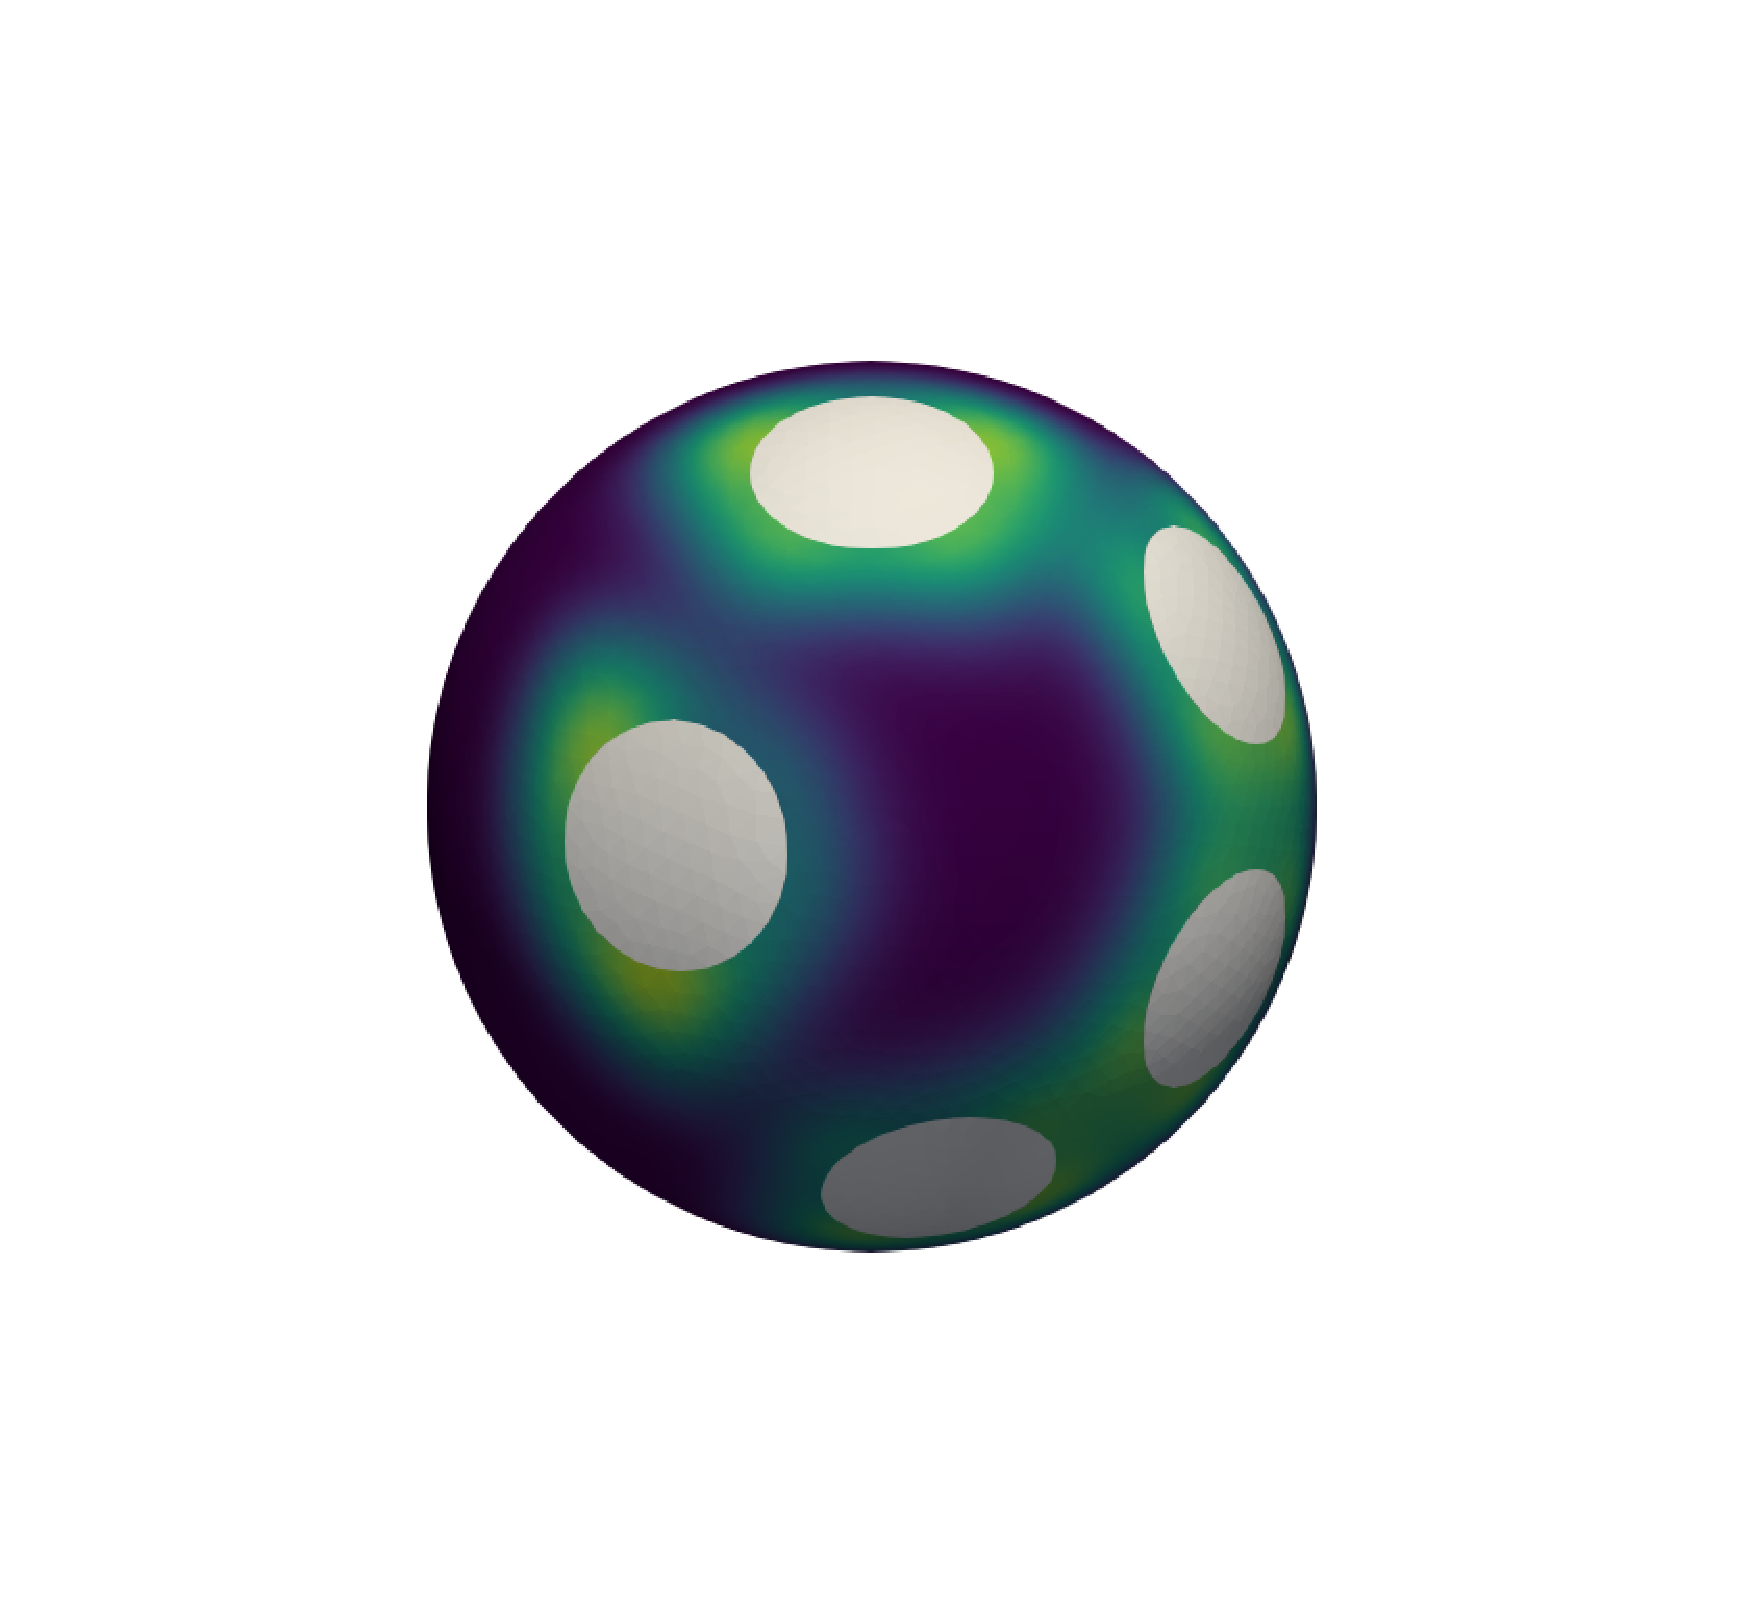
\includegraphics[scale=0.178]{./Pictures/p1.eps}};
%====================================================================
% Classic
\node[inner sep=0pt] at (3,0)
    {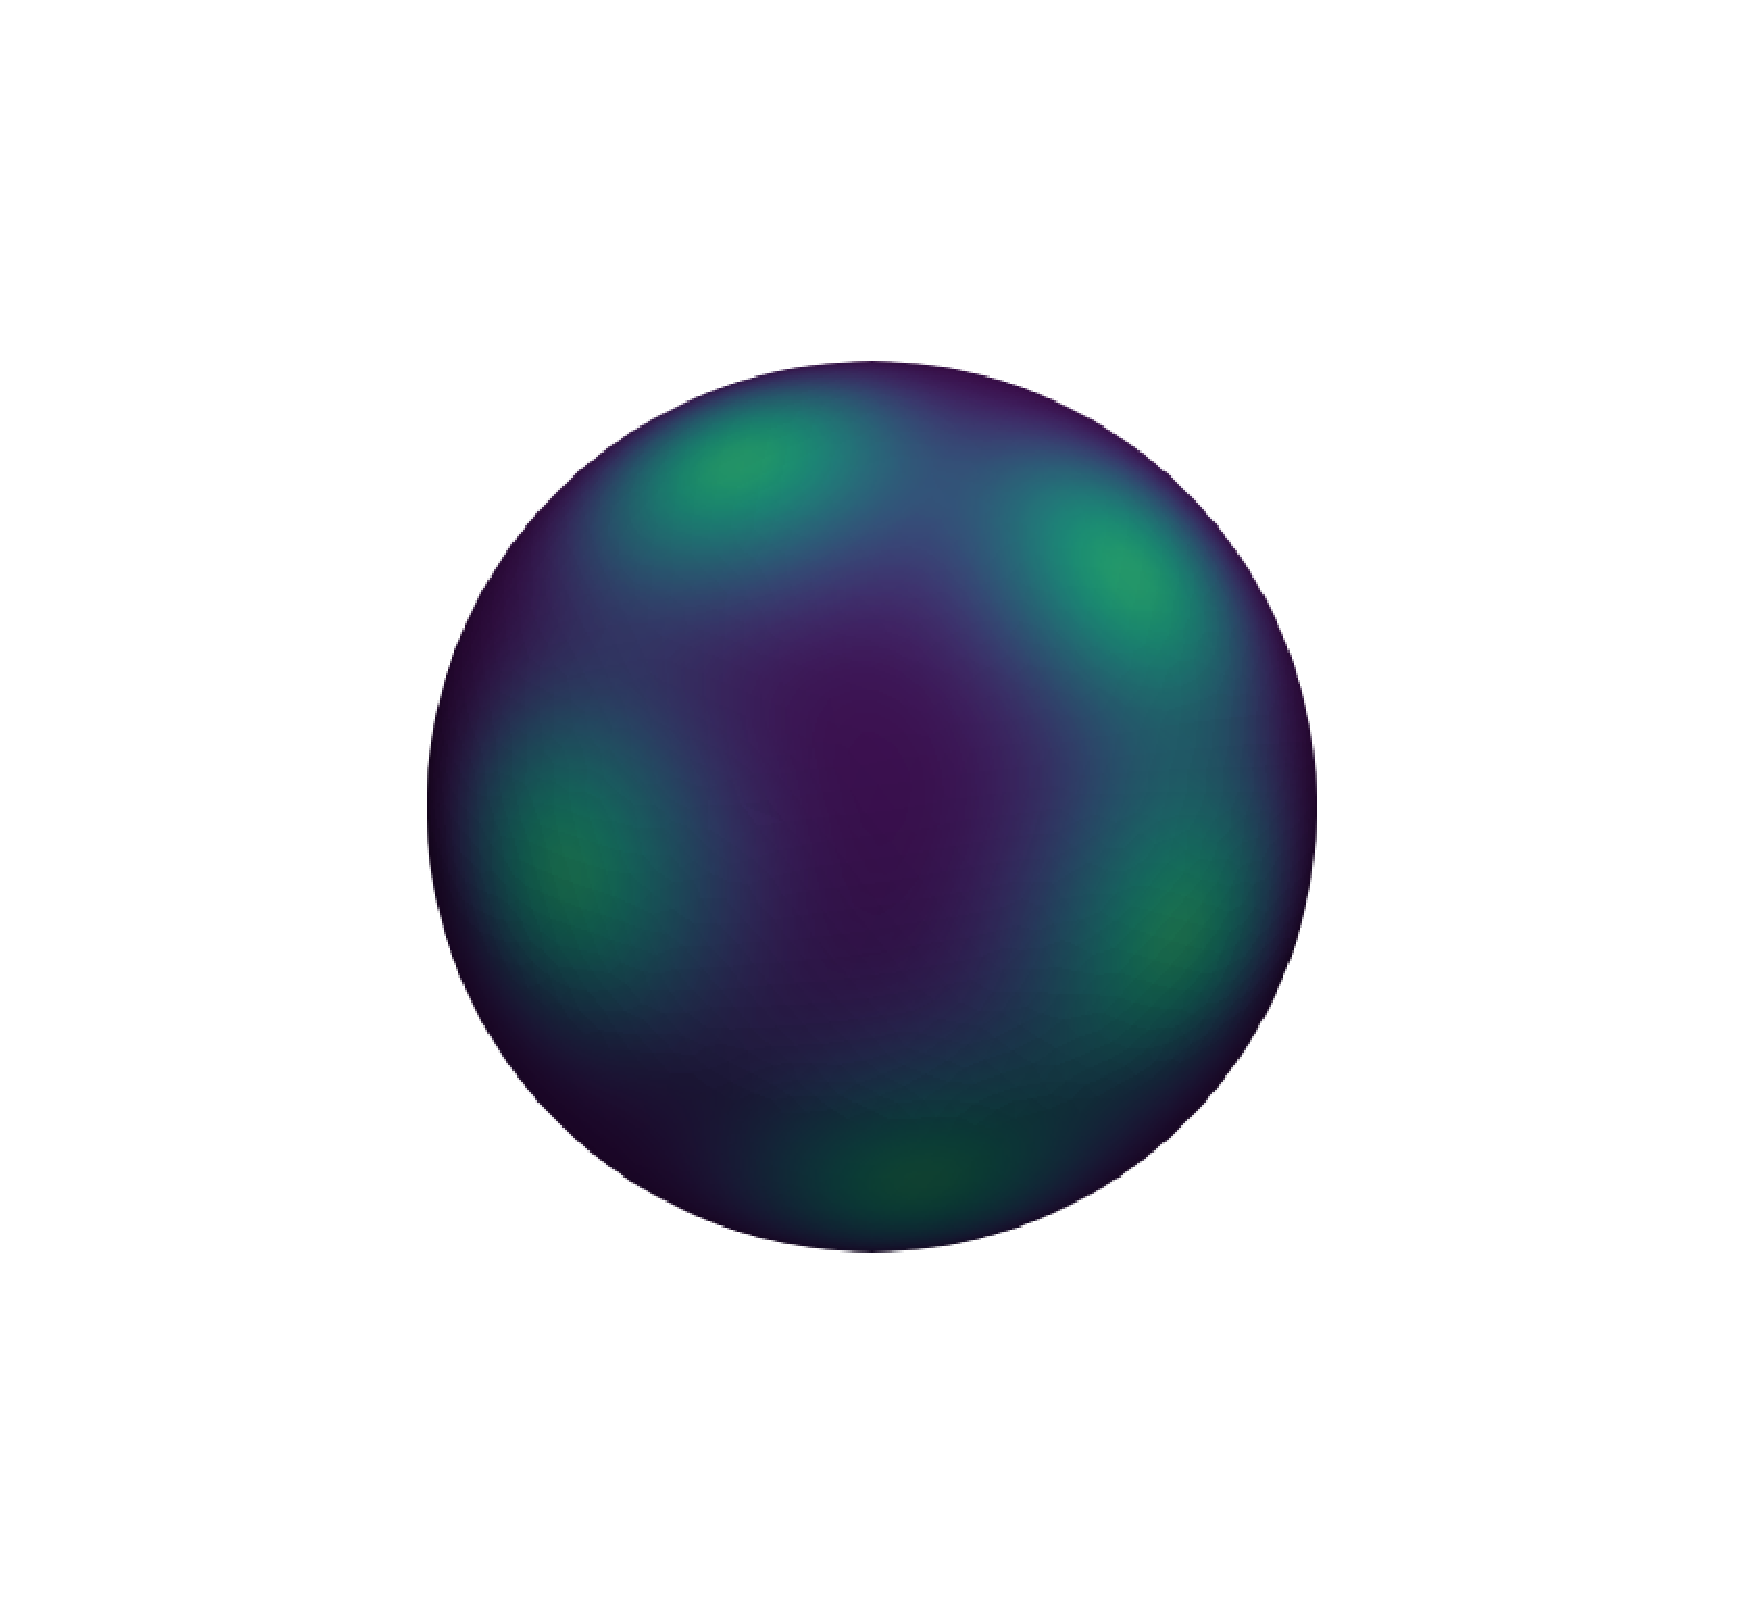
\includegraphics[scale=0.178]{./Pictures/v2.eps}};
% Non-classic
\node[inner sep=0pt] at (3,-6)
    {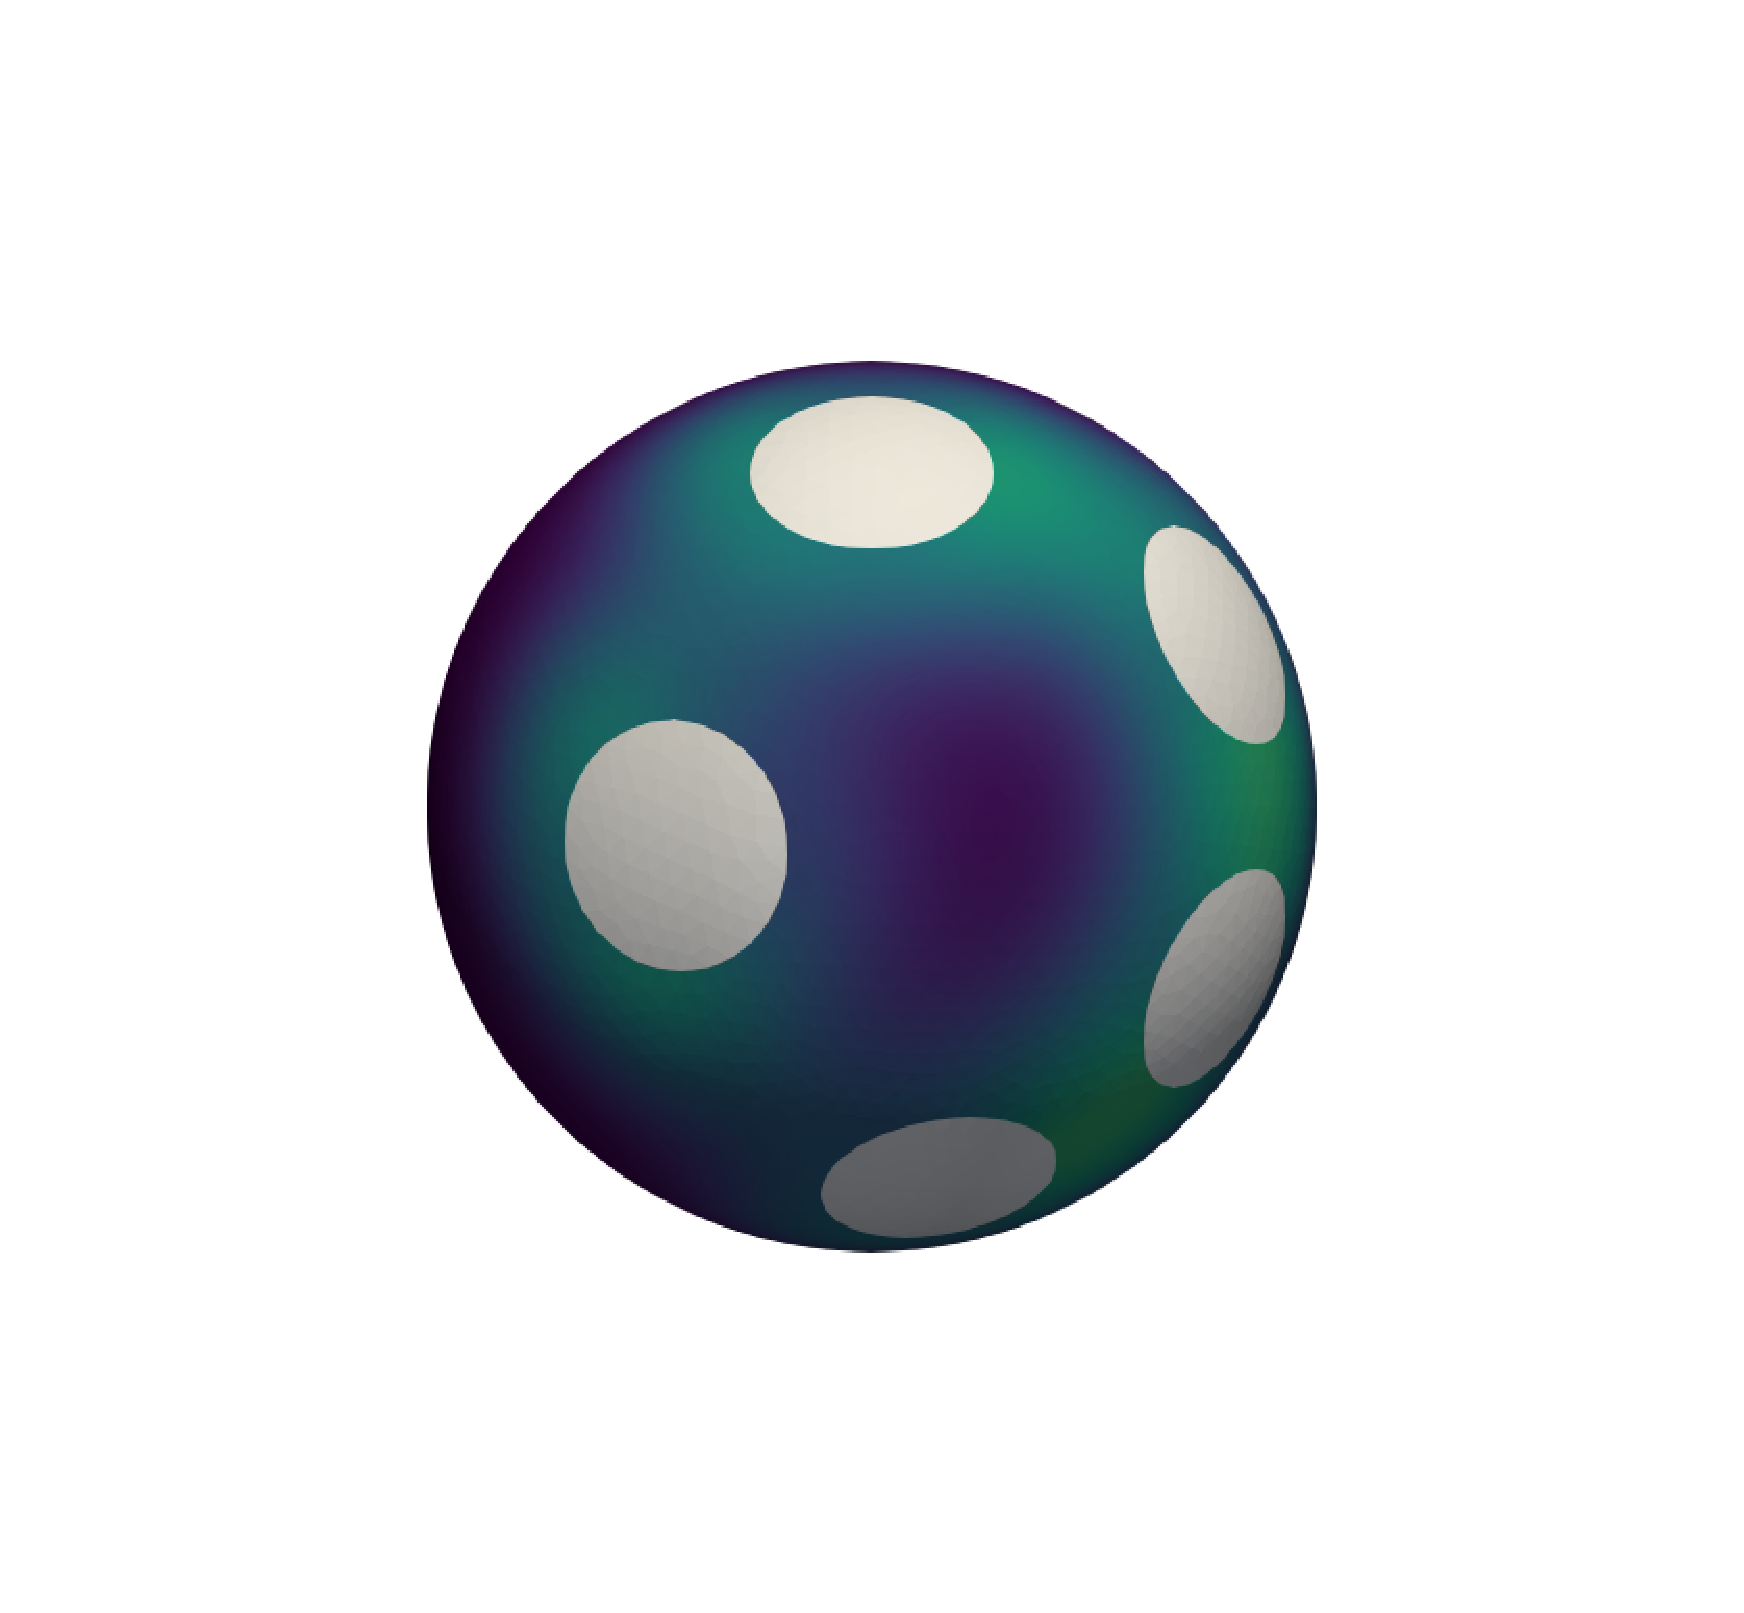
\includegraphics[scale=0.178]{./Pictures/p2.eps}};
%====================================================================
% Classic
\node[inner sep=0pt] at (9,0)
    {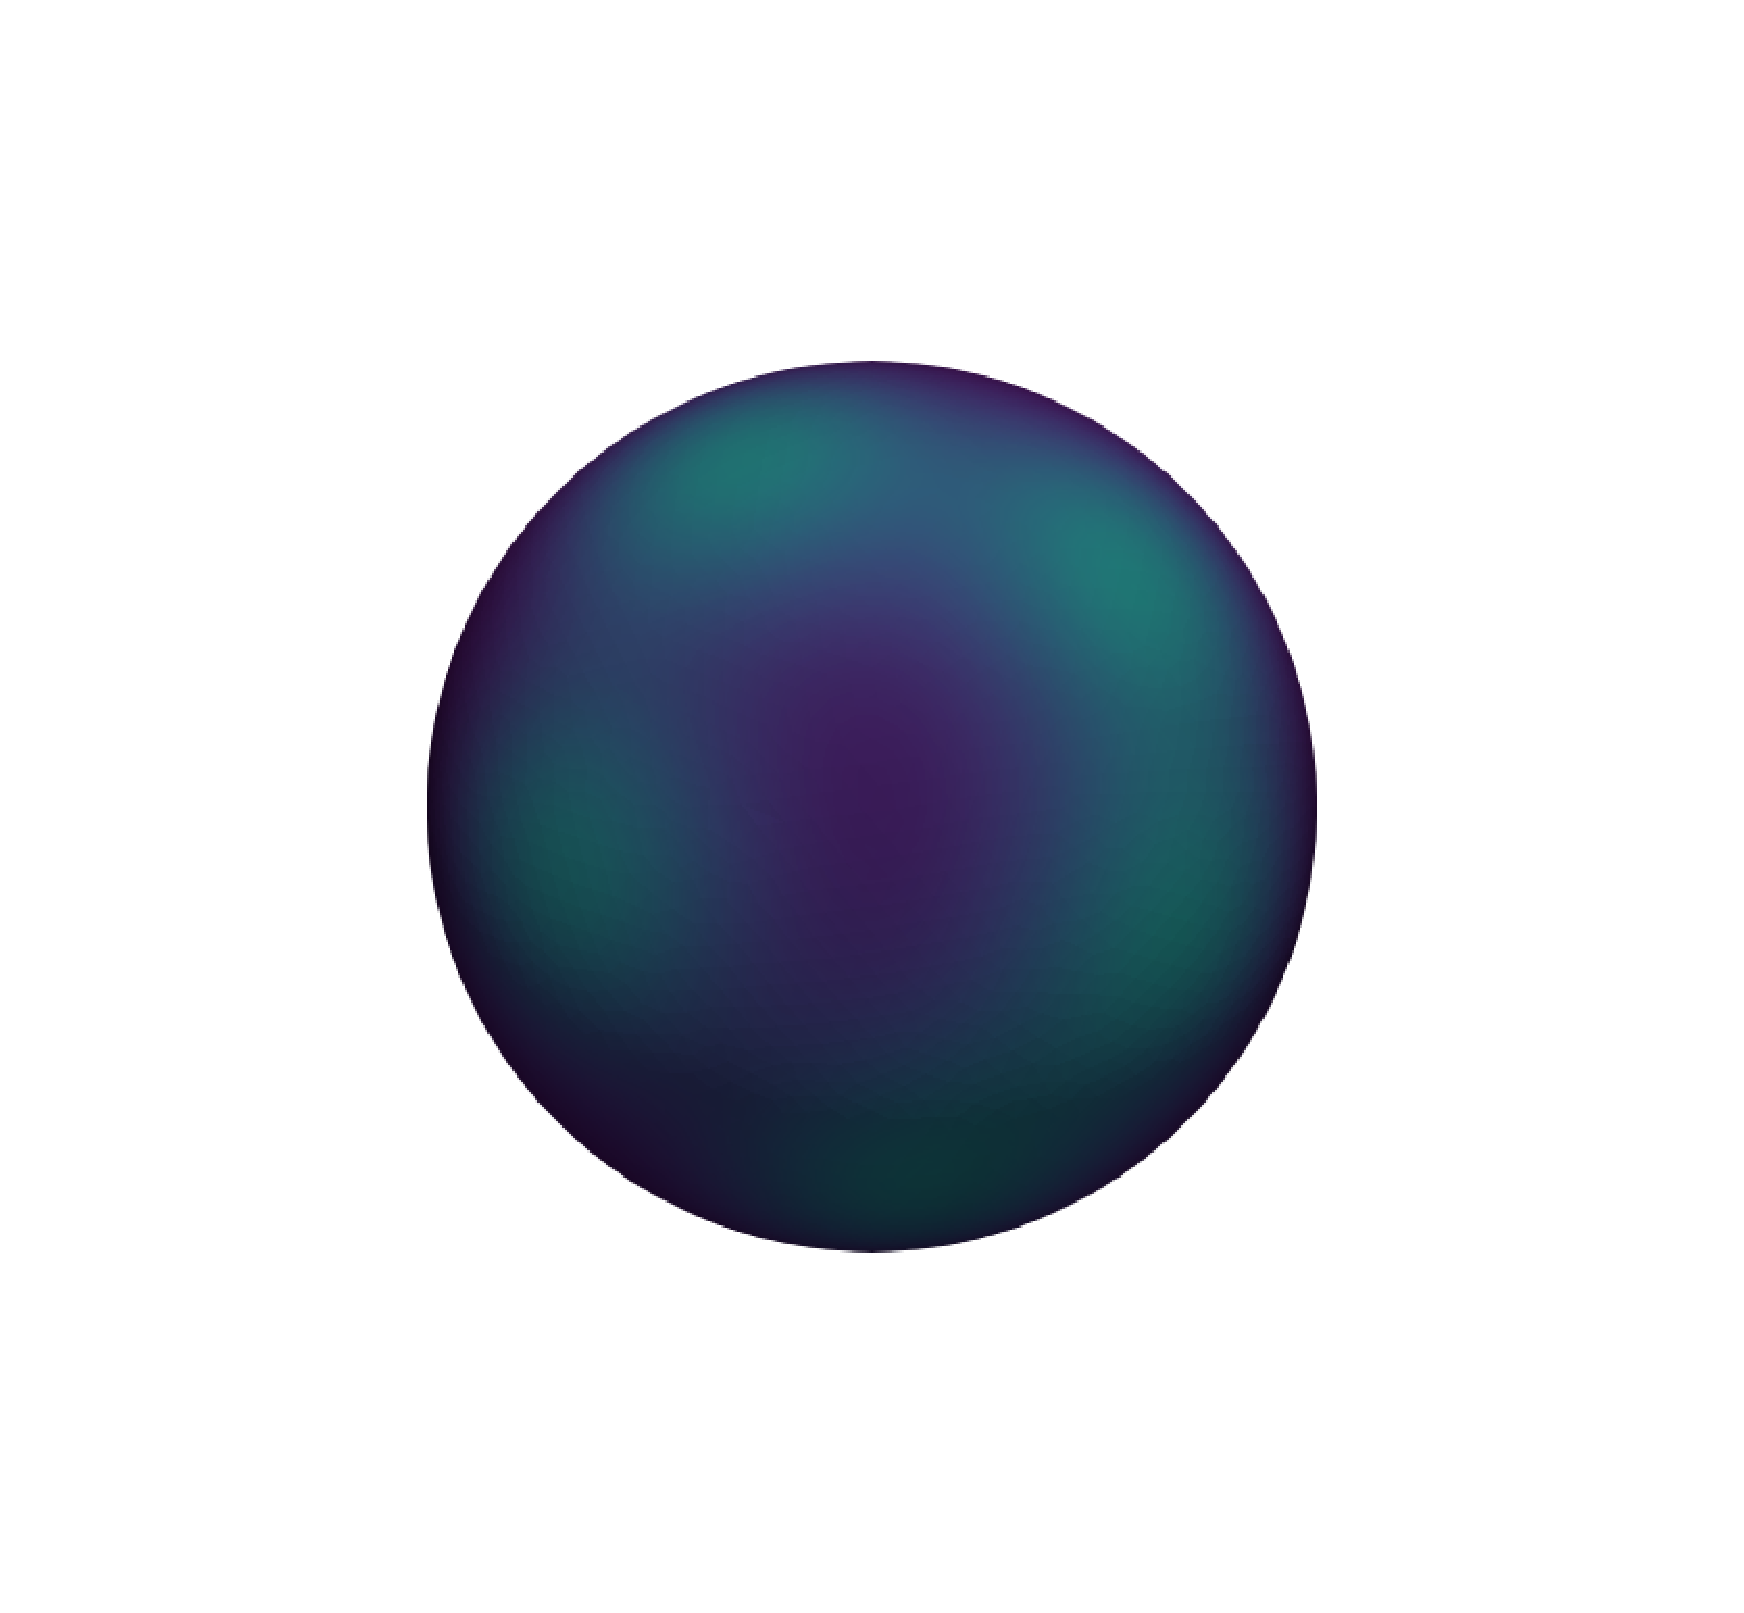
\includegraphics[scale=0.178]{./Pictures/v3.eps}};
% Non-classic
\node[inner sep=0pt] at (9,-6)
    {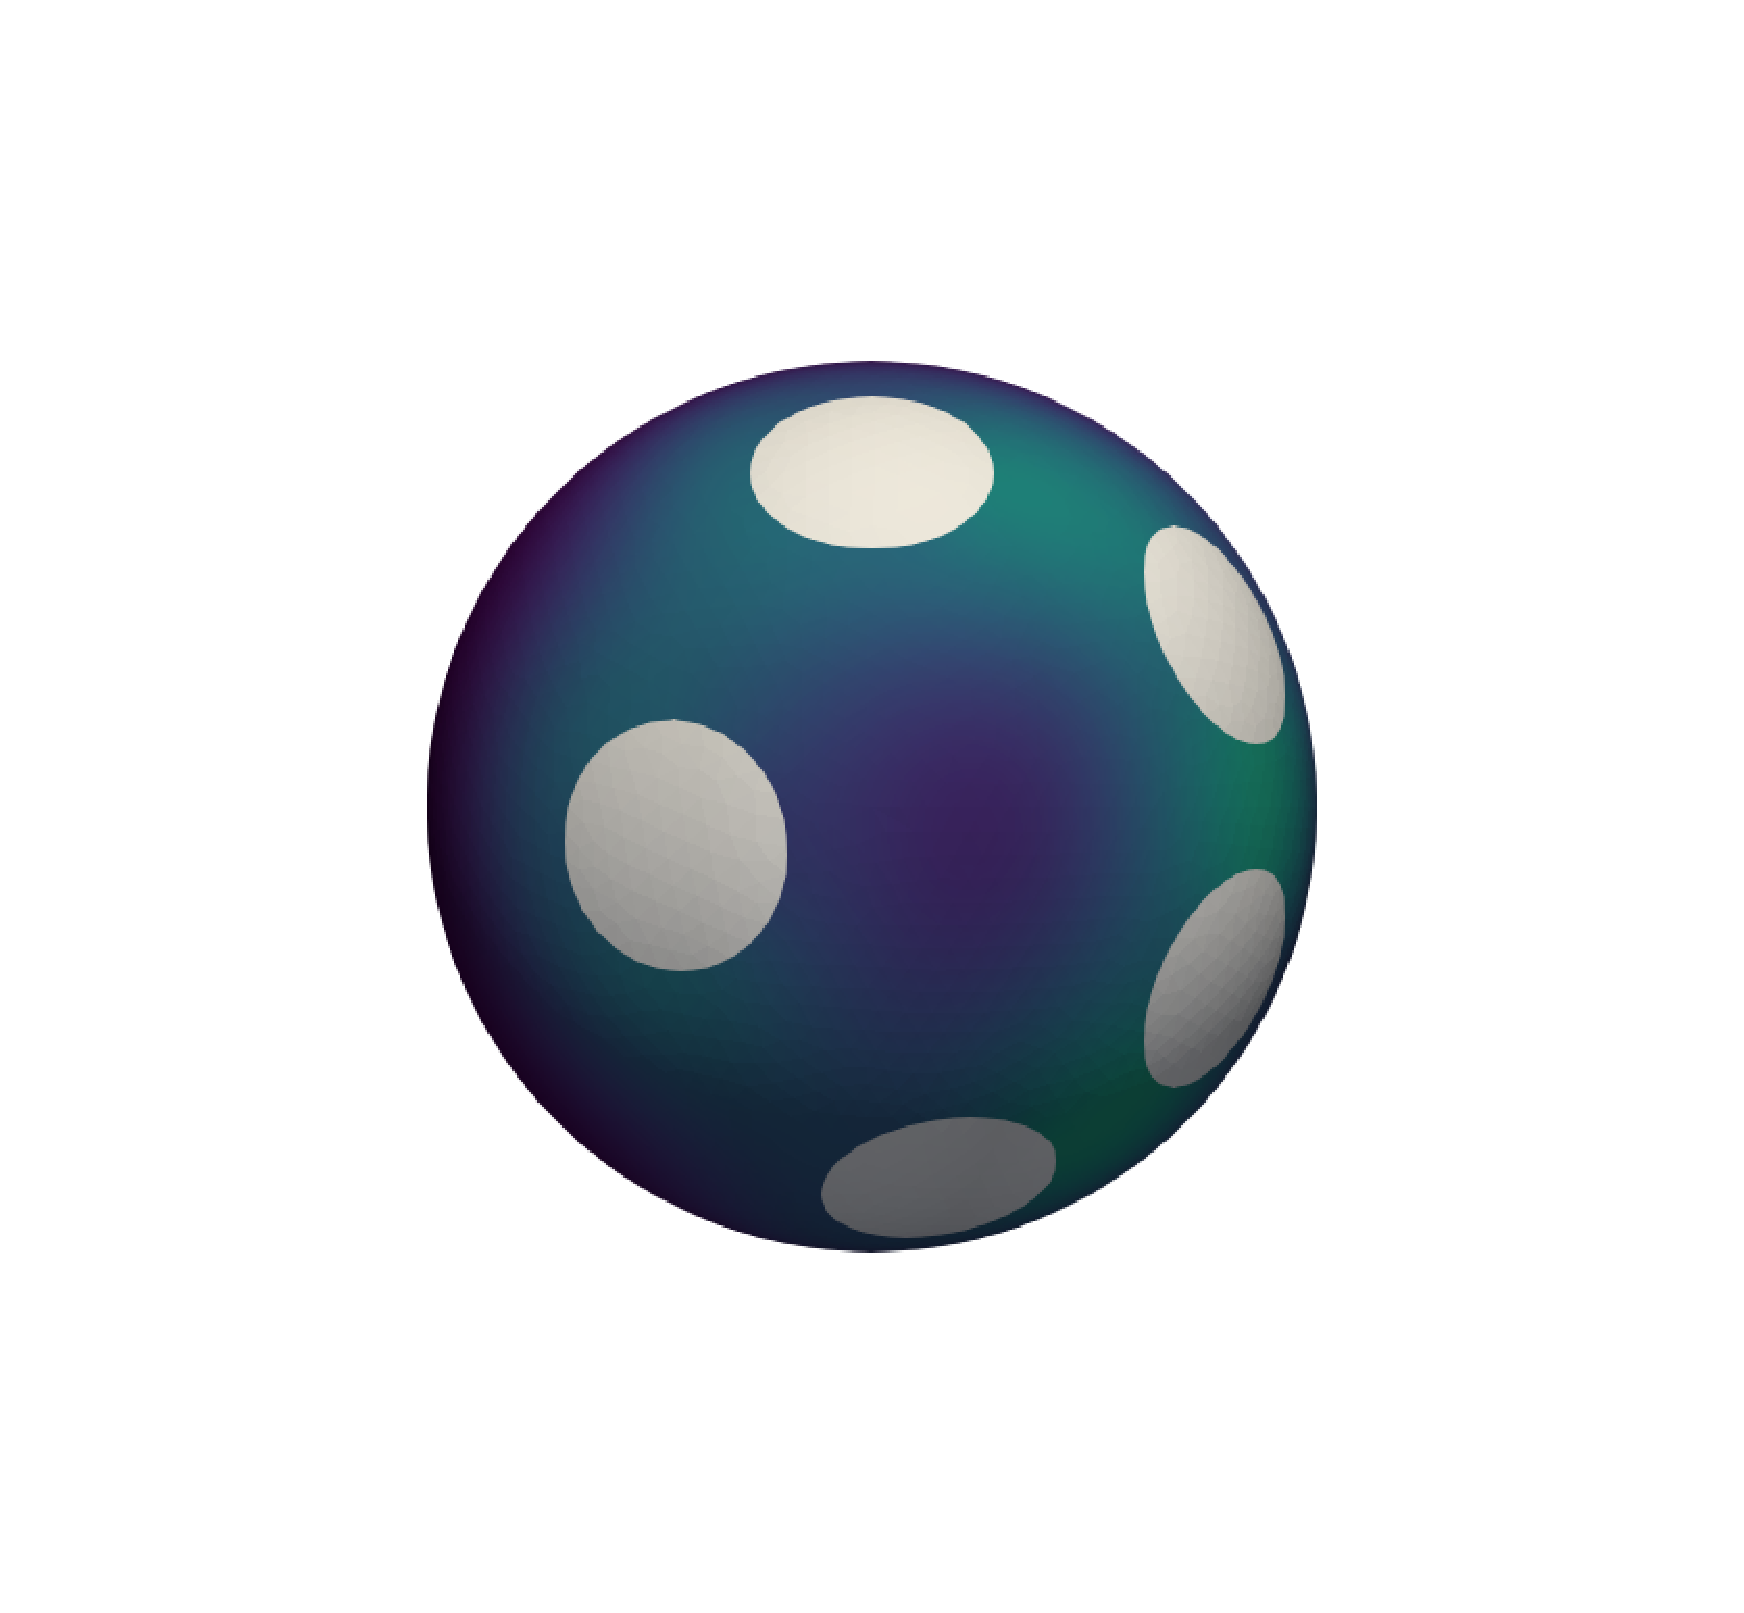
\includegraphics[scale=0.178]{./Pictures/p3.eps}};
%====================================================================
% Classic
\node[inner sep=0pt] at (15,0)
    {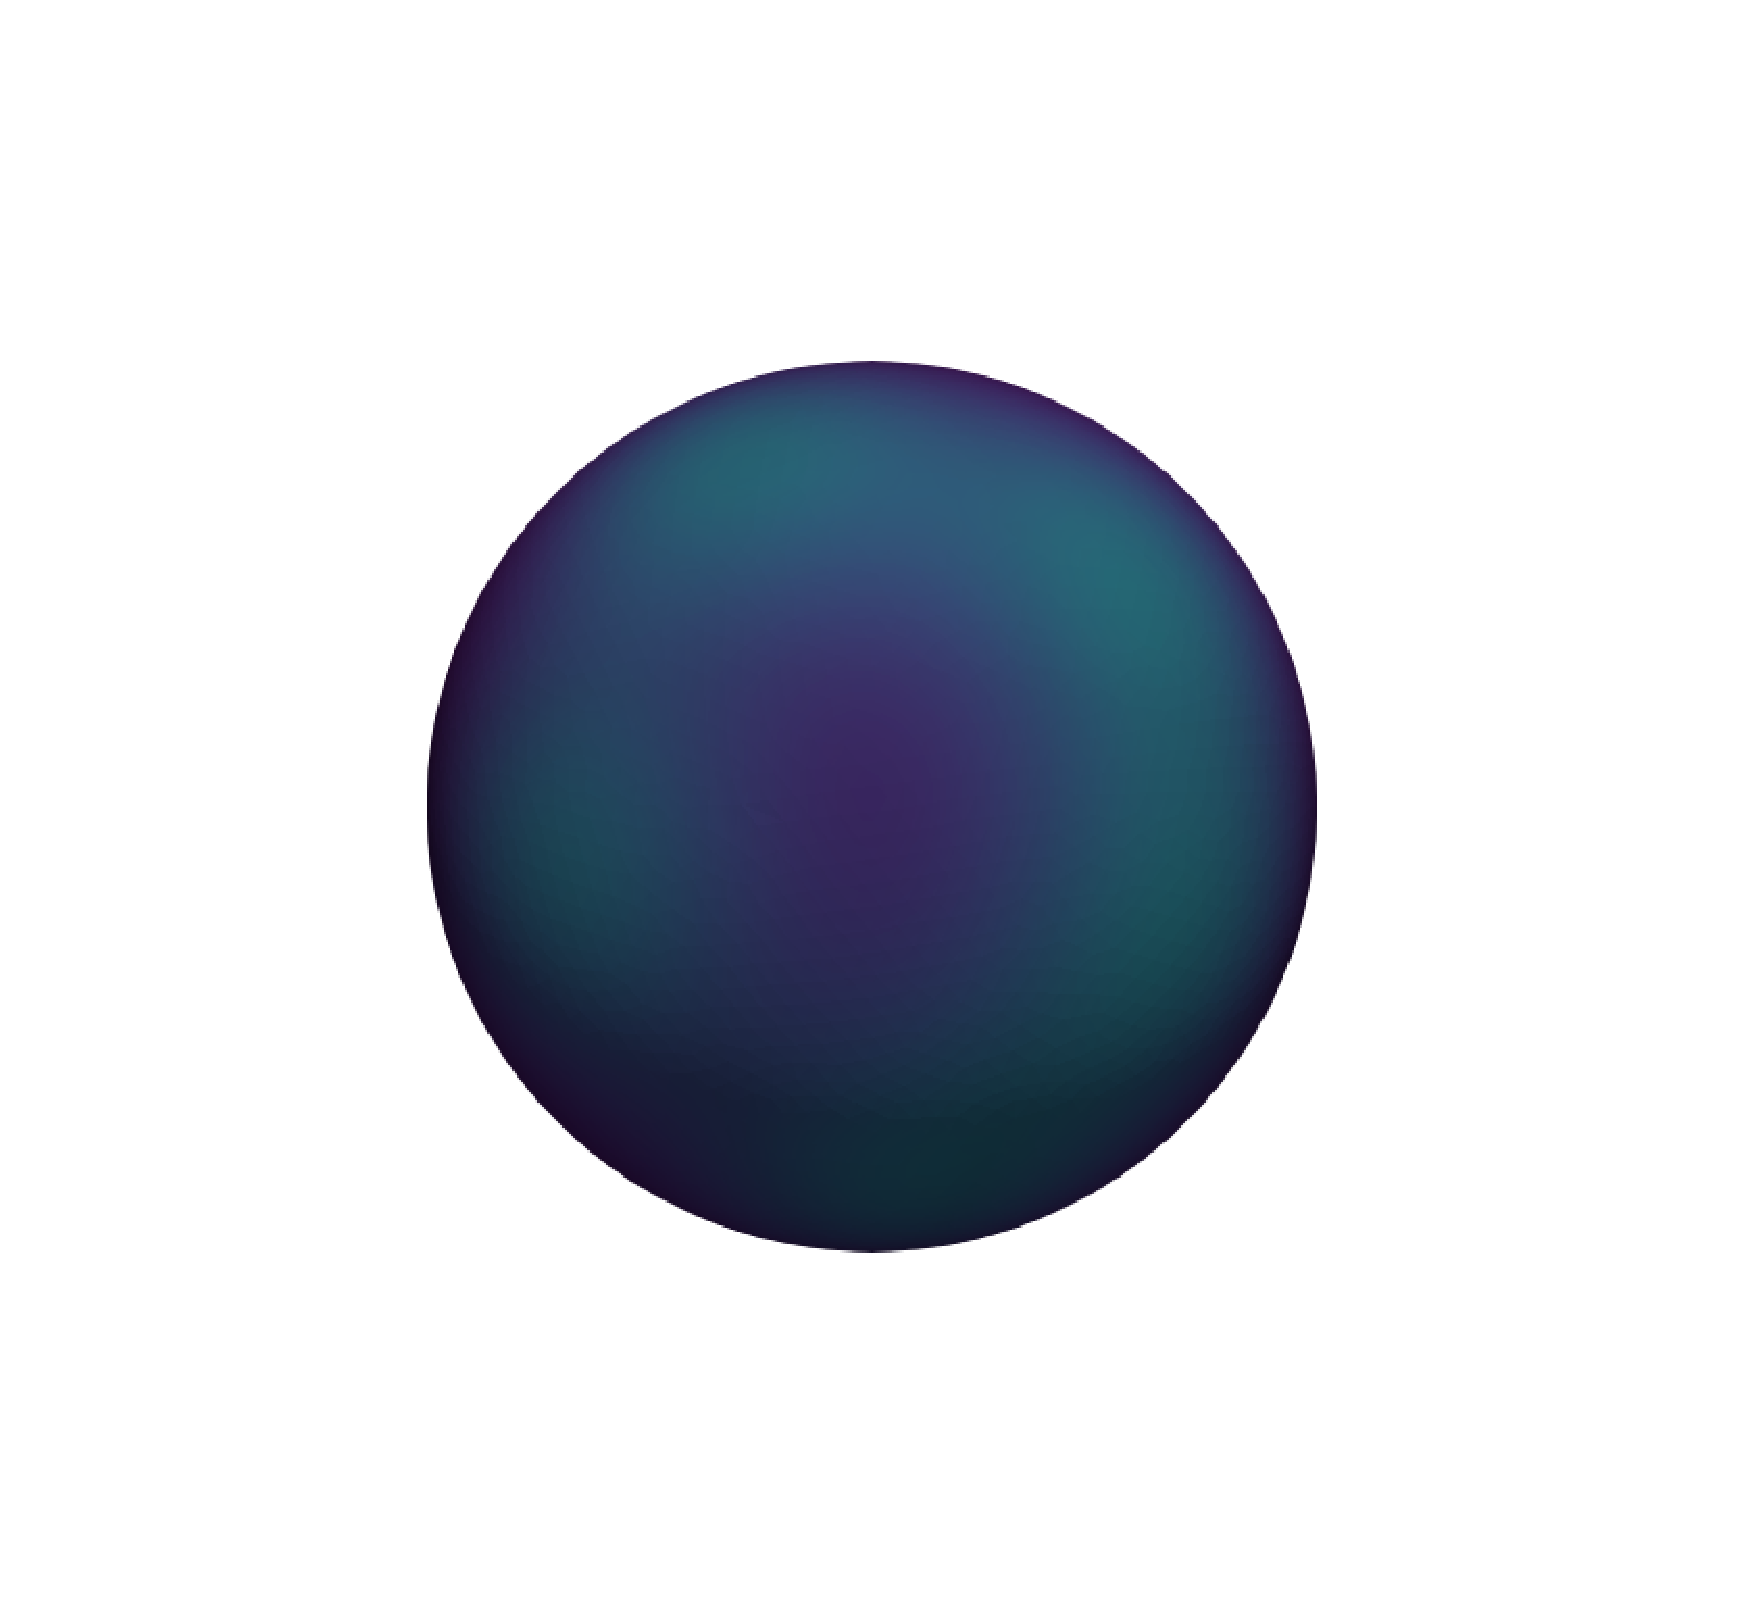
\includegraphics[scale=0.178]{./Pictures/v4.eps}};
% Non-classic
\node[inner sep=0pt] at (15,-6)
    {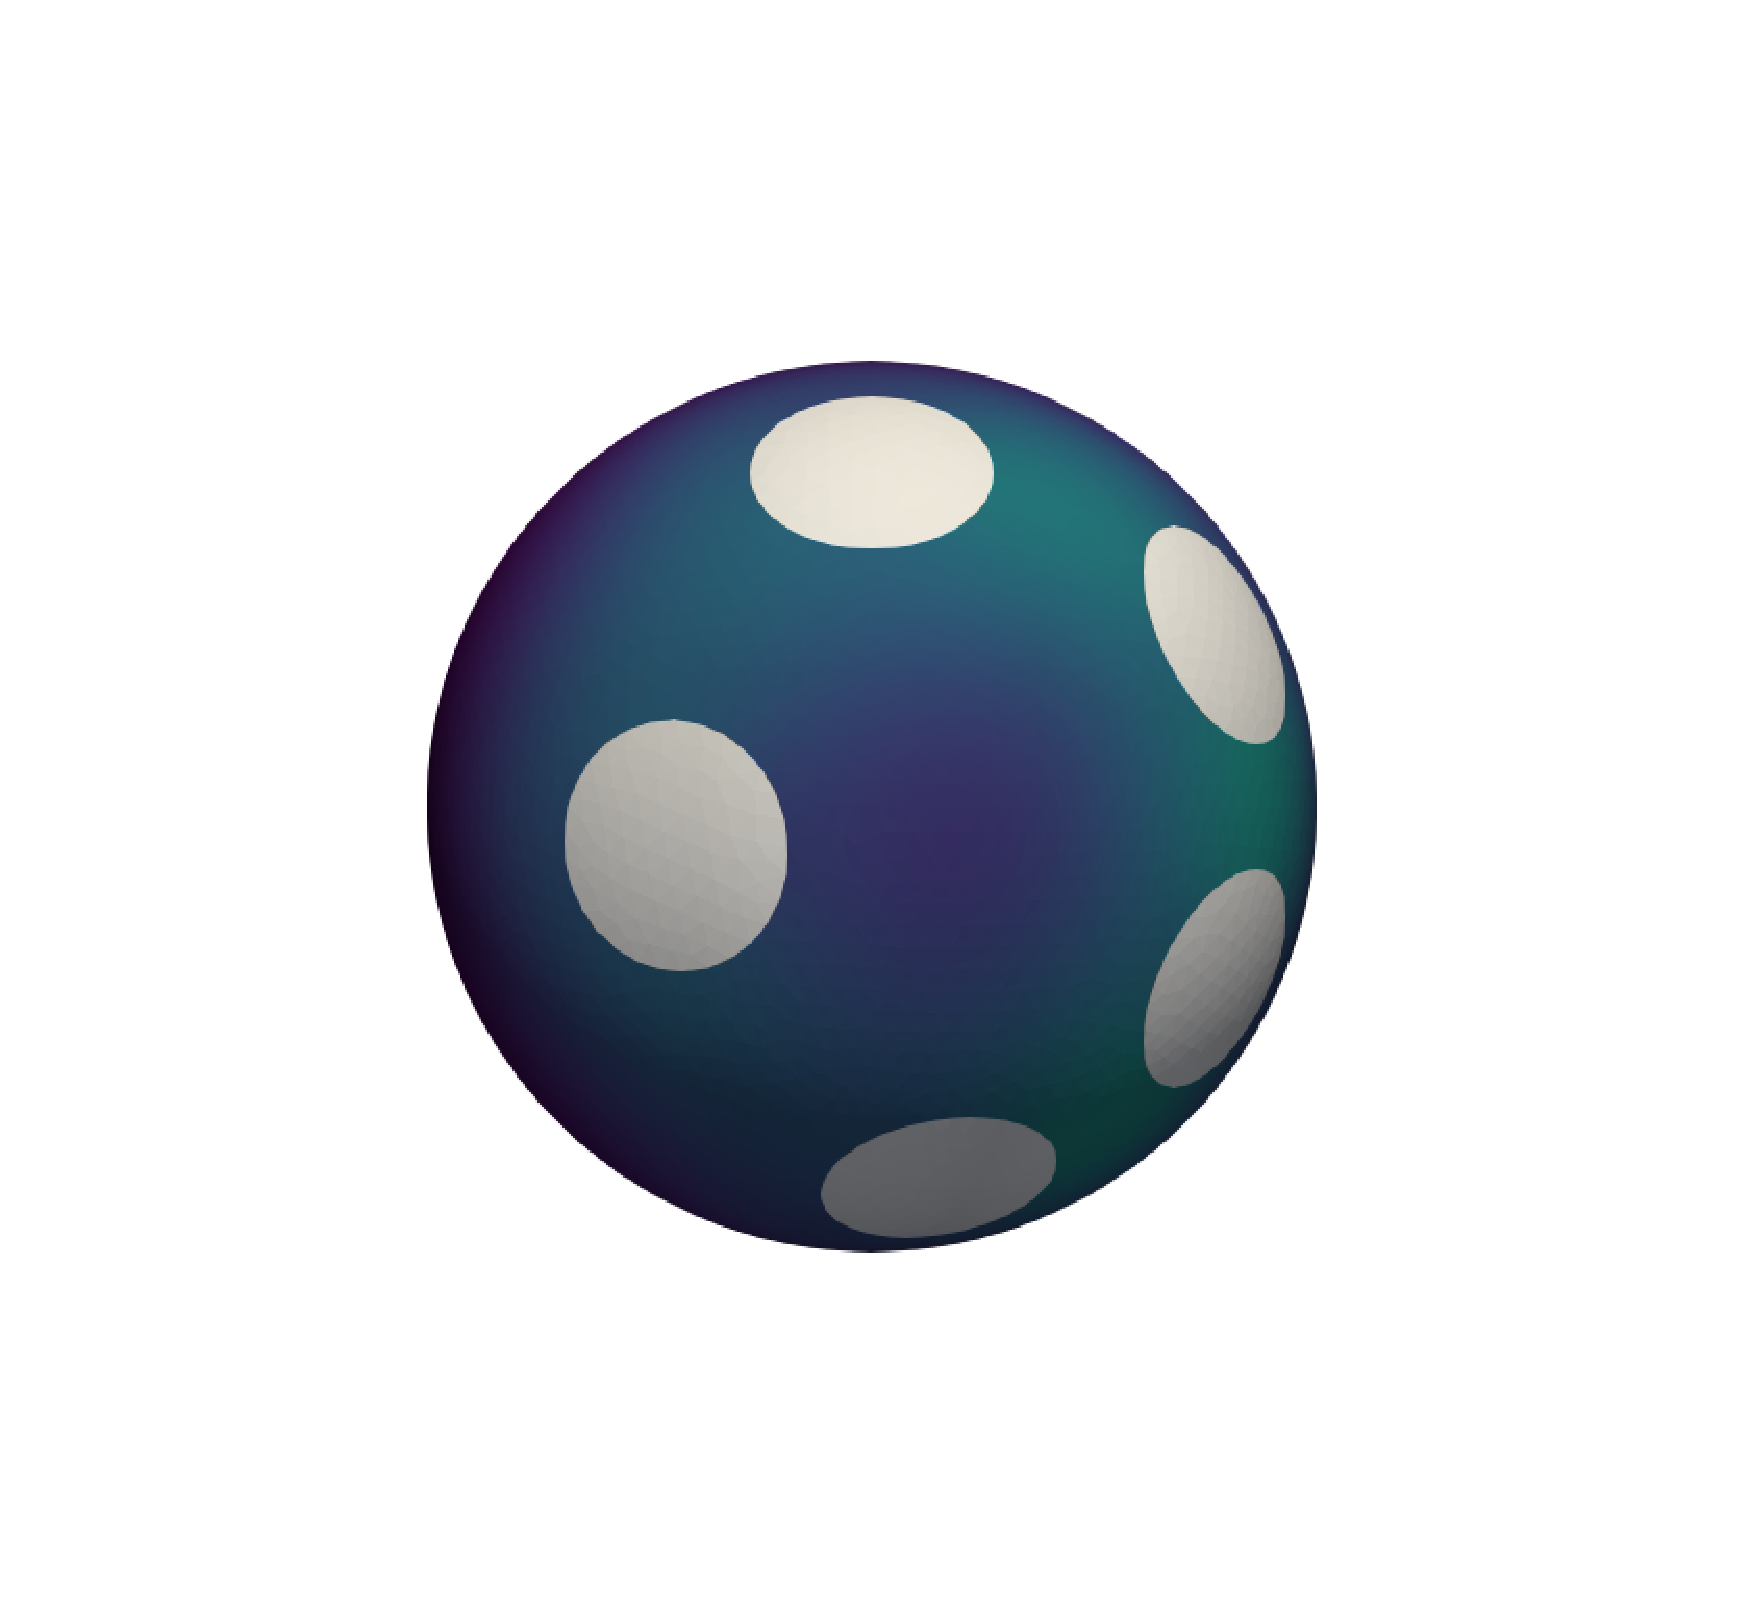
\includegraphics[scale=0.178]{./Pictures/p4.eps}};
%====================================================================
% ADD (A) AND (B)
\node at (-12,1) {\huge\textit{(B1)}};
\node at (-12,-5.00) {\huge\textit{(B2)}};
\draw [->,ultra thick,line width=2mm,-latex] (-10,-10) -- (17,-10);
\node at (4,-11) {\huge\textit{Increasing time,} $t$};     
%====================================================================
% VERTICAL COLOURBAR
\node[inner sep=0pt] at (18.5,-3.25)
    {
\includegraphics[scale=0.45,angle =0]{./Pictures/colourbar.eps}};
    \node[align=center] at (20.25,-7.2) {\Large\textbf{$u_{\min}$}/\textbf{$v_{\min}$}};
    \node[align=center] at (20.25,1.2) {\Large\textbf{$u_{\max}$}/\textbf{$v_{\max}$}};
    % TO MAKE SURE EVERYTHING IS IN LINE: UNCOMMENT TO SEE
    %\draw [-,ultra thick,line width=2mm] (-13,1.75) -- (22,1.75);
    %\draw [-,ultra thick,line width=2mm] (-13,-7.75) -- (22,-7.75);
    %\draw [-,ultra thick,line width=2mm] (-13,-4.25) -- (22,-4.25);
%====================================================================
% HORIZONTAL COLOURBAR
%\node[inner sep=0pt] at (2,7)
%    {
\includegraphics[scale=1.2,angle =90]{./Pictures/colourbar.eps}};
%    \node at (14,4.2) {\Huge\textbf{$0$}};
%    \node at (-11,4.2) {\Huge\textbf{$u_{\max}$}};

%====================================================================
% WE PUT ALL PARAMETERS AFTERWARDS SO THAT WE CAN OVERWRITE IMAGES
%====================================================================
%CLASSIC CASE
\node at (-9,-2.75) { \Large$t=0$};
\node at (-3,-2.75) { \Large$t\approx 0.006$};
\node at (3,-2.75) { \Large$t\approx 0.018$};
\node at (9,-2.75) {\Large$t\approx 0.031$};
\node at (15,-2.75) {\Large$t\approx 0.043$};
% Smaller labels
%\node at (-9,2.0) { \huge (A.1)};
%\node at (-3,2.0) { \huge (A.2)};
%\node at (3,2.0) { \huge (A.3)};
%\node at (9,2.0) {\huge (A.4)};
%\node at (15,2.0) {\huge (A.5)};
%NON-CLASSIC CASE
\node at (-9,-8.75) { \Large$t=0$};
\node at (-3,-8.75) { \Large$t\approx 0.006$};
\node at (3,-8.75) { \Large$t\approx 0.018$};
\node at (9,-8.75) { \Large$t\approx 0.031$};
\node at (15,-8.75) {\Large$t\approx 0.043$};
% Smaller labels
%\node at (-9,-4.00) { \huge (B.1)};
%\node at (-3,-4.00) { \huge (B.2)};
%\node at (3,-4.00) { \huge (B.3)};
%\node at (9,-4.00) {\huge (B.4)};
%\node at (15,-4.00) {\huge (B.5)};
\end{tikzpicture}

\end{document}